% Options for packages loaded elsewhere
\PassOptionsToPackage{unicode}{hyperref}
\PassOptionsToPackage{hyphens}{url}
%
\documentclass[
]{article}
\usepackage{amsmath,amssymb}
\usepackage{lmodern}
\usepackage{iftex}
\ifPDFTeX
  \usepackage[T1]{fontenc}
  \usepackage[utf8]{inputenc}
  \usepackage{textcomp} % provide euro and other symbols
\else % if luatex or xetex
  \usepackage{unicode-math}
  \defaultfontfeatures{Scale=MatchLowercase}
  \defaultfontfeatures[\rmfamily]{Ligatures=TeX,Scale=1}
\fi
% Use upquote if available, for straight quotes in verbatim environments
\IfFileExists{upquote.sty}{\usepackage{upquote}}{}
\IfFileExists{microtype.sty}{% use microtype if available
  \usepackage[]{microtype}
  \UseMicrotypeSet[protrusion]{basicmath} % disable protrusion for tt fonts
}{}
\makeatletter
\@ifundefined{KOMAClassName}{% if non-KOMA class
  \IfFileExists{parskip.sty}{%
    \usepackage{parskip}
  }{% else
    \setlength{\parindent}{0pt}
    \setlength{\parskip}{6pt plus 2pt minus 1pt}}
}{% if KOMA class
  \KOMAoptions{parskip=half}}
\makeatother
\usepackage{xcolor}
\usepackage[margin=1in]{geometry}
\usepackage{longtable,booktabs,array}
\usepackage{calc} % for calculating minipage widths
% Correct order of tables after \paragraph or \subparagraph
\usepackage{etoolbox}
\makeatletter
\patchcmd\longtable{\par}{\if@noskipsec\mbox{}\fi\par}{}{}
\makeatother
% Allow footnotes in longtable head/foot
\IfFileExists{footnotehyper.sty}{\usepackage{footnotehyper}}{\usepackage{footnote}}
\makesavenoteenv{longtable}
\usepackage{graphicx}
\makeatletter
\def\maxwidth{\ifdim\Gin@nat@width>\linewidth\linewidth\else\Gin@nat@width\fi}
\def\maxheight{\ifdim\Gin@nat@height>\textheight\textheight\else\Gin@nat@height\fi}
\makeatother
% Scale images if necessary, so that they will not overflow the page
% margins by default, and it is still possible to overwrite the defaults
% using explicit options in \includegraphics[width, height, ...]{}
\setkeys{Gin}{width=\maxwidth,height=\maxheight,keepaspectratio}
% Set default figure placement to htbp
\makeatletter
\def\fps@figure{htbp}
\makeatother
\setlength{\emergencystretch}{3em} % prevent overfull lines
\providecommand{\tightlist}{%
  \setlength{\itemsep}{0pt}\setlength{\parskip}{0pt}}
\setcounter{secnumdepth}{5}
\usepackage{lineno}
% \linenumbers
\usepackage{float}
\ifLuaTeX
  \usepackage{selnolig}  % disable illegal ligatures
\fi
\usepackage[]{natbib}
\bibliographystyle{plainnat}
\IfFileExists{bookmark.sty}{\usepackage{bookmark}}{\usepackage{hyperref}}
\IfFileExists{xurl.sty}{\usepackage{xurl}}{} % add URL line breaks if available
\urlstyle{same} % disable monospaced font for URLs
\hypersetup{
  pdftitle={Implications of Measurement Errors in Water Use Estimates for Water Management},
  pdfauthor={Taro Mieno; Timothy Foster; Nicholas Brozovic},
  hidelinks,
  pdfcreator={LaTeX via pandoc}}

\title{Implications of Measurement Errors in Water Use Estimates for Water Management}
\author{Taro Mieno\footnote{Department of Agricultural Economics, University of Nebraska Lincoln, \href{mailto:tmieno2@unl.edu}{\nolinkurl{tmieno2@unl.edu}}} \and Timothy Foster\footnote{Department of WWW, University of Manchester, \href{mailto:timothy.foster@manchester.ac.uk}{\nolinkurl{timothy.foster@manchester.ac.uk}}} \and Nicholas Brozovic\footnote{Department of Agricultural Economics, University of Nebraska Lincoln, \href{mailto:nbrozovic@nebraska.edu}{\nolinkurl{nbrozovic@nebraska.edu}}}}
\date{}

\begin{document}
\maketitle
\begin{abstract}
abstract here
\end{abstract}

\hypertarget{main}{%
\section{Main}\label{main}}

\hypertarget{background}{%
\subsection{Background}\label{background}}

\begin{itemize}
\tightlist
\item
  intensity estimation accuracy
\item
  (estimated) intensity-based vs (estimated) area-based (Southern Europe History)
\item
  (estimated) intensity-based vs (true) intensity-based {[}We work on this{]}
\end{itemize}

key objective:

\begin{itemize}
\item
  start a discussion about the implications of the use of mis-measured water use for water use regulation.
\item
  shed lights on unintentional consequences of using estiamtes rather than actual measurements
\end{itemize}

Two policies:
+ water quota (examples of existing quota systems)
+ water permit trading

Lack of measurement. Emergence of Open ET as a substitute.

No clear policy design suggestions on how to use water use estiamtes with measurement errors.

\hypertarget{results}{%
\section{Results}\label{results}}

\hypertarget{profit-under-water-and-proxy-quota}{%
\subsection{Profit under water and proxy quota}\label{profit-under-water-and-proxy-quota}}

Figure \ref{fig:profit-quota-water-het} below compares profit from agricultural production as a function of actual water use between water and proxy quota across three different production heterogeneity levels. When there is no heterogeneity in farmers' production function, water quota is the most cost effective way to achieve a water use reduction goal (highest profit achievable for a given level of actual water use). Under this circumstance, proxy quota with unbiased measurement errors achieves worse than water quota due to asymmetry in downside and upside risk of water use.

\begin{figure}[H]

{\centering 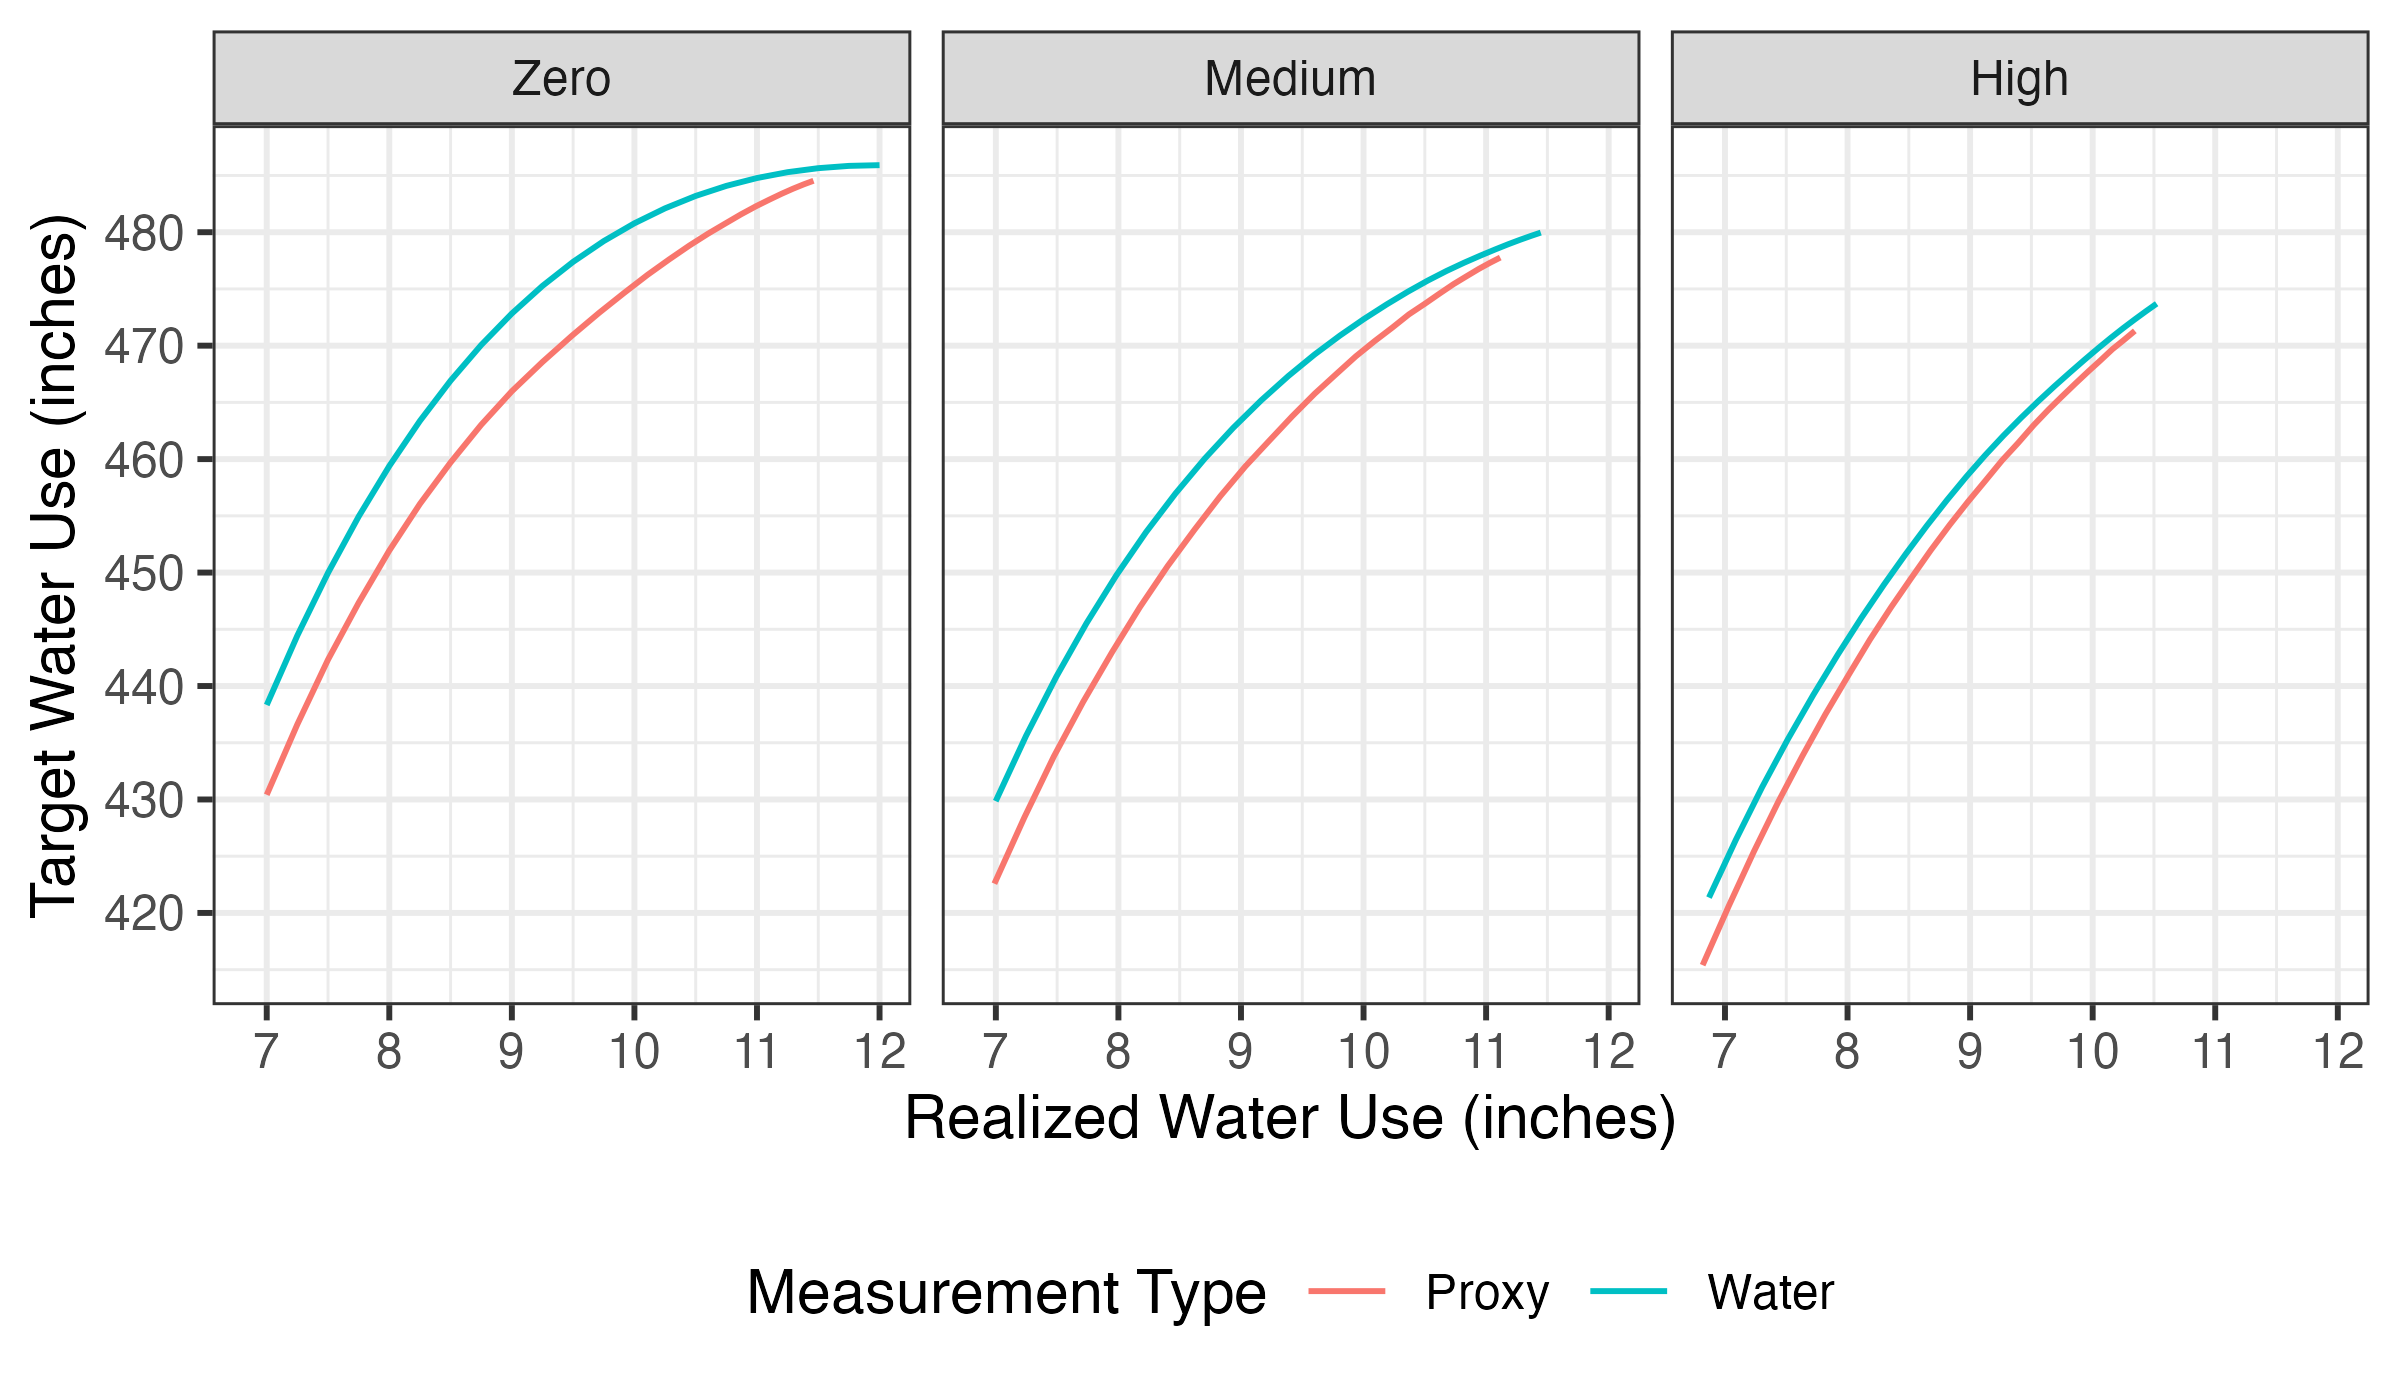
\includegraphics{figures/g_profit_quota_w_vs_p} 

}

\caption{Comparison of profit from agricultural production between the water and quota systems}\label{fig:profit-quota-water-het}
\end{figure}

Figure \ref{fig:illust-homegeneous} presents an illustration to build the intuition behind the profit loss due to the use of proxy quota in place of water quota. The red dotted lines indicate the effective water use quota. Under the water quota system, both farmers receive 7 inches of water quota. Since the unconstrained profit maximizing water use is 10.94 inches, both farmers use up all the allocated quota and use 10 inches of water. Under the proxy quota system, they are allocated the same amount of proxy quota. However, measurement error in proxy quota resulted in effective water quota of 4 and 10 inches for farmer A and B, respectively. Both farmers use their allocated amout of water. Under both proxy and water quota systems, the total water use is 14 inches. Farmer B makes 30.6035744 less under the water quota system compared to the proxy quota system. However, Farmer A makes 133.2697115 more under the water quota system compared to the proxy quota system. This comes from an important nature of crop production with respsect to water: declining marginal impact of water on crop yield. As can be seen in the profit-water relationship, removing an inch of water from 6 inches has much larger negative impact compared to revmoing an inch of water from 10 inches.

\begin{figure}[H]

{\centering 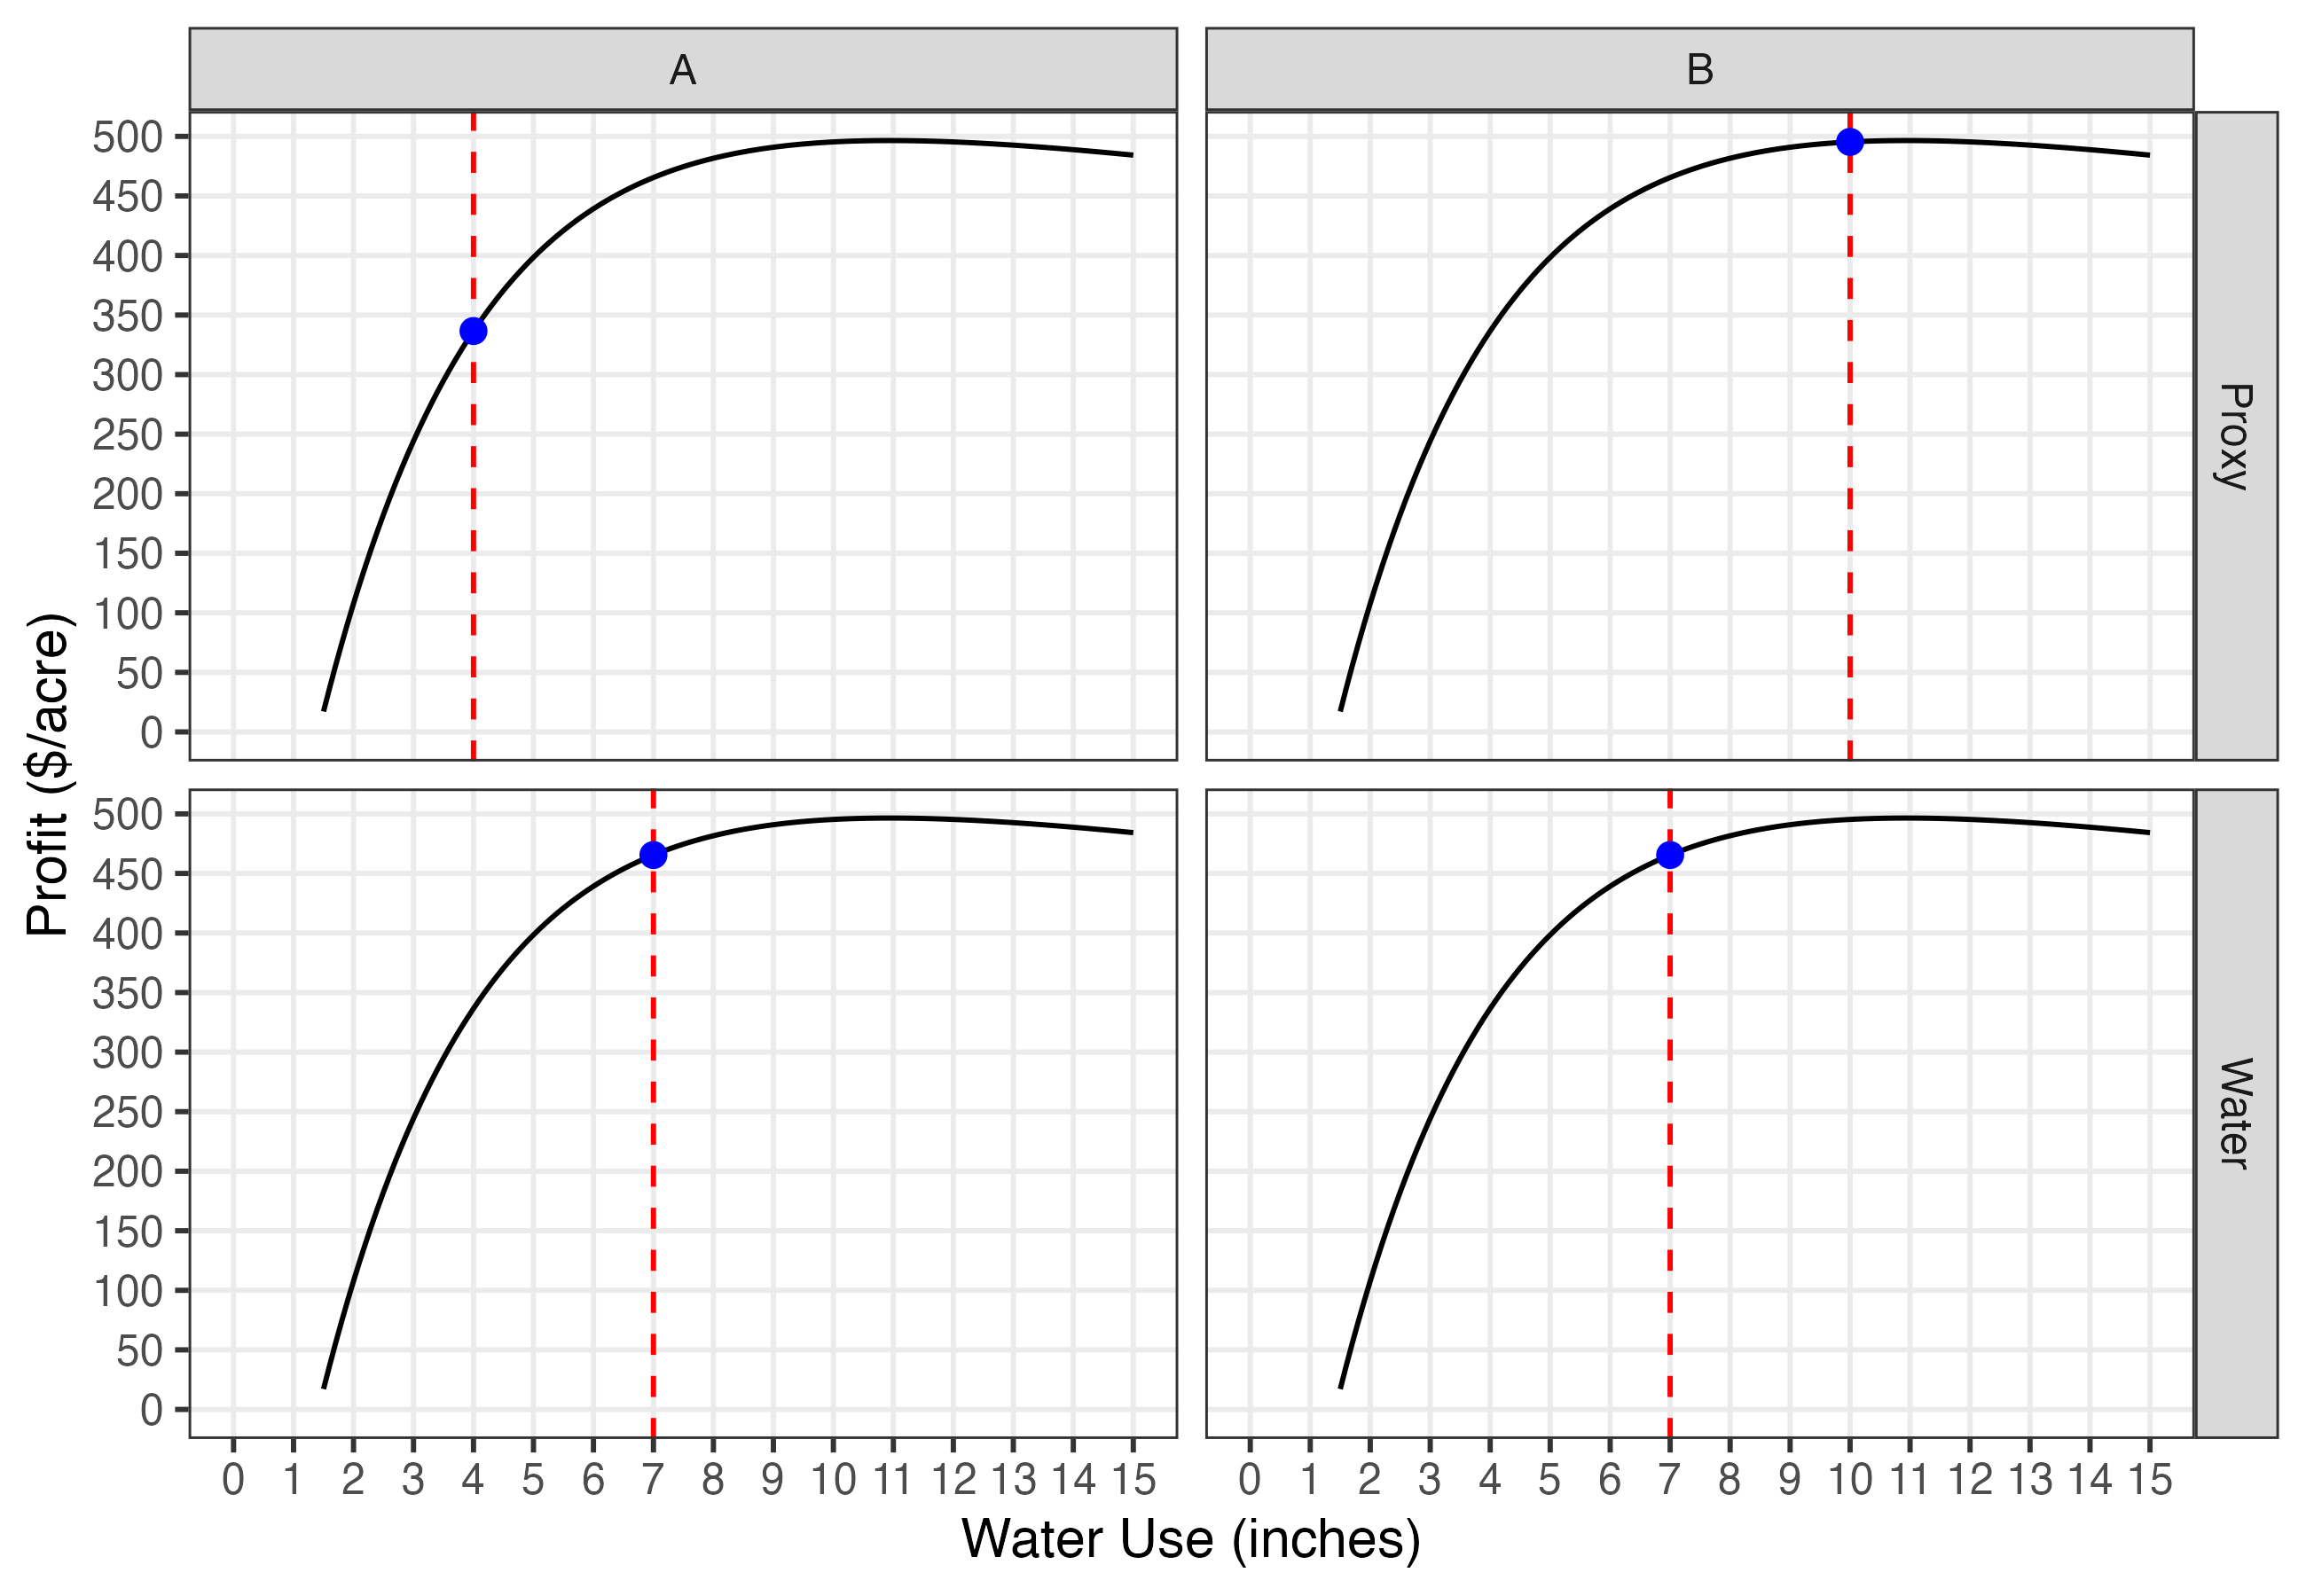
\includegraphics{figures/g_illustration_homogeneous} 

}

\caption{Illustration of profit loss due to the use of proxy for quota-based regulation: a case of homegeneous producers}\label{fig:illust-homegeneous}
\end{figure}

However, as the heterogeneity of farmers increases, comparative advantage of water quota over proxy quota diminishes. While the performance of both systems declines as the level of heterogeneity increases, water quota is affected more so than the proxy quota system. This is because uniform quota now acts like heterogeneous quota under homogeneous production function because the same quota is given to farmers with heterogeneous water demand. This is illustrated in Figure \ref{fig:illust-heterogeneous}. In this example, farmer A needs less water than farmer B. Water and proxy quota allocated to the farmers are exactly the same as the previous case. In this example, errors in proxy happened to realize so that more effective water quota is given to farmer B than farmer A. Consequently, proxy quota produces a higher total profit than water quota. Of course, if error happened to go the opposite way, then the performance of proxy quota relative to water quota is even worse compared to the homogeneous case. This is a big contrast to the homogeneous case because water quota is always better than proxy quota in that case. Consequently, proxy quota performs relatively better under heterogeneous cases. On average, the positive and negative effects of measurement errors tend to even out. However, proxy quota is never better than water quota \textbf{on average} (see Appendix \ldots{} for mathematical proof).

\begin{figure}[H]

{\centering 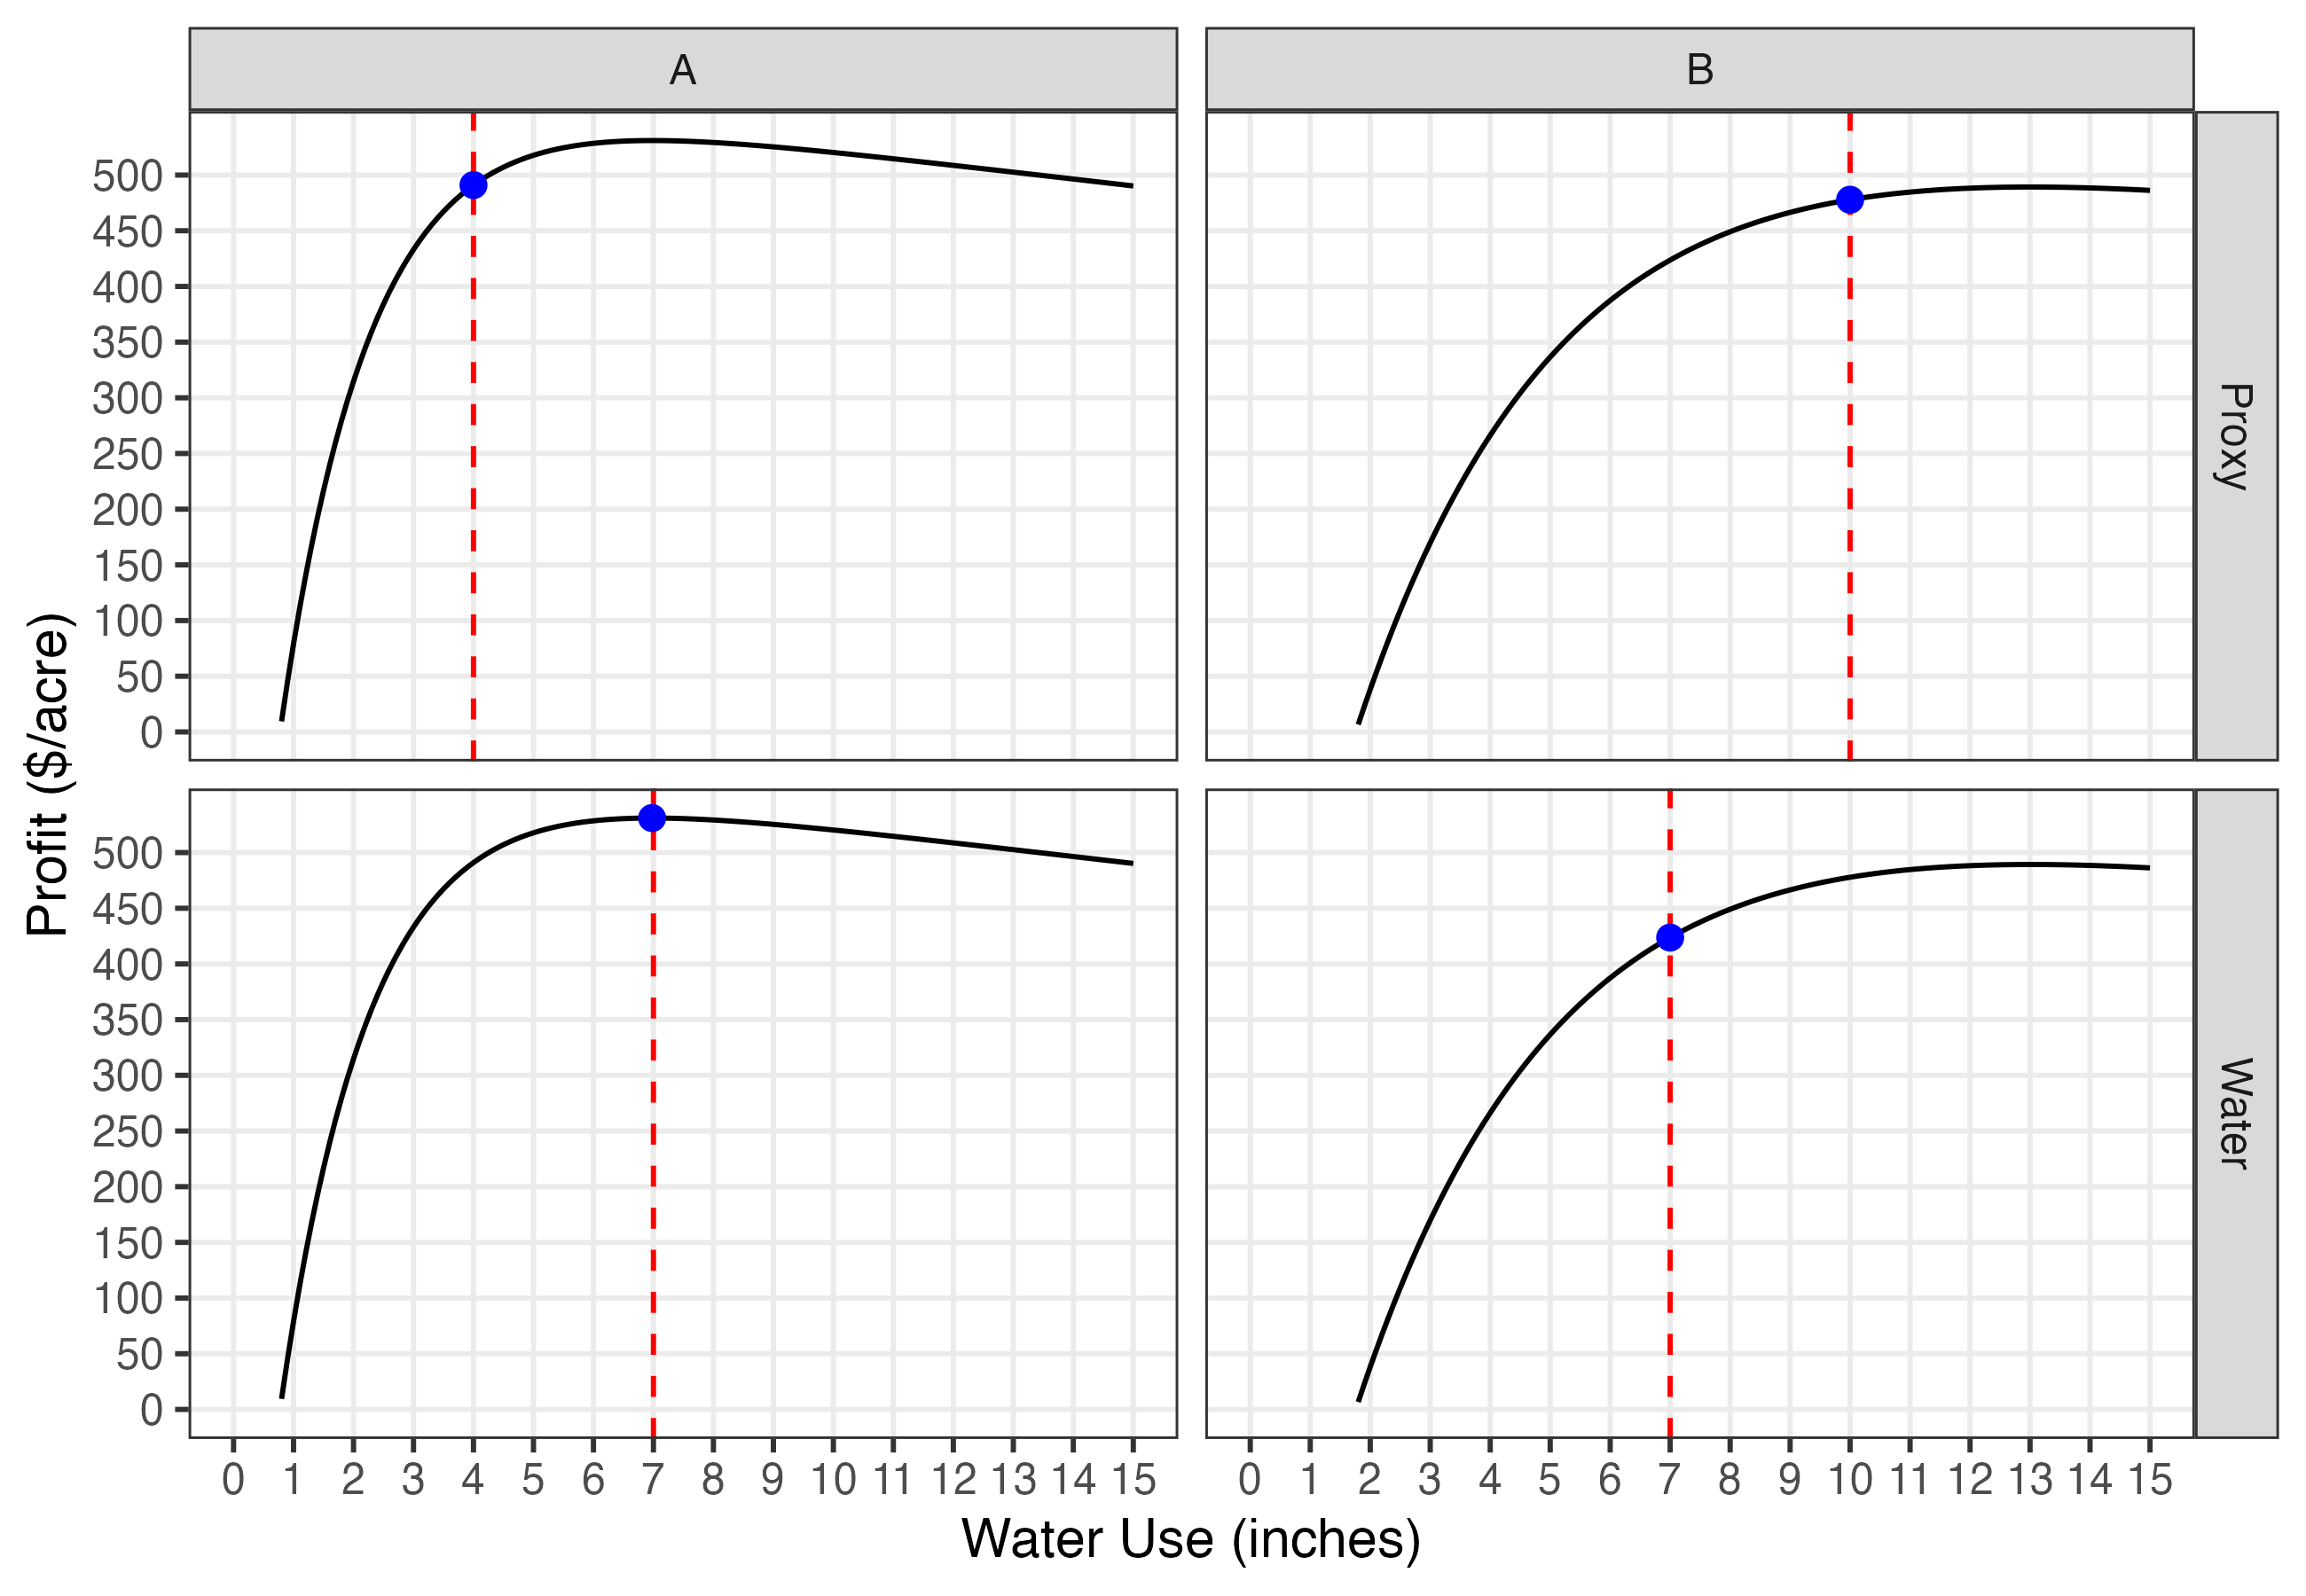
\includegraphics{figures/g_illustration_het} 

}

\caption{Illustration of profit loss due to the use of proxy for quota-based regulation: a case of heterogeneous producers}\label{fig:illust-heterogeneous}
\end{figure}

When measurement error is independent and production function is concave, water quota always outperforms proxy quota (show proof in appendix).

\hypertarget{the-effect-of-increasing-the-size-of-measurement-error}{%
\subsection{The effect of increasing the size of measurement error}\label{the-effect-of-increasing-the-size-of-measurement-error}}

\textbf{Convert $u\_dev$ to $R^2$.}

\begin{figure}[H]

{\centering 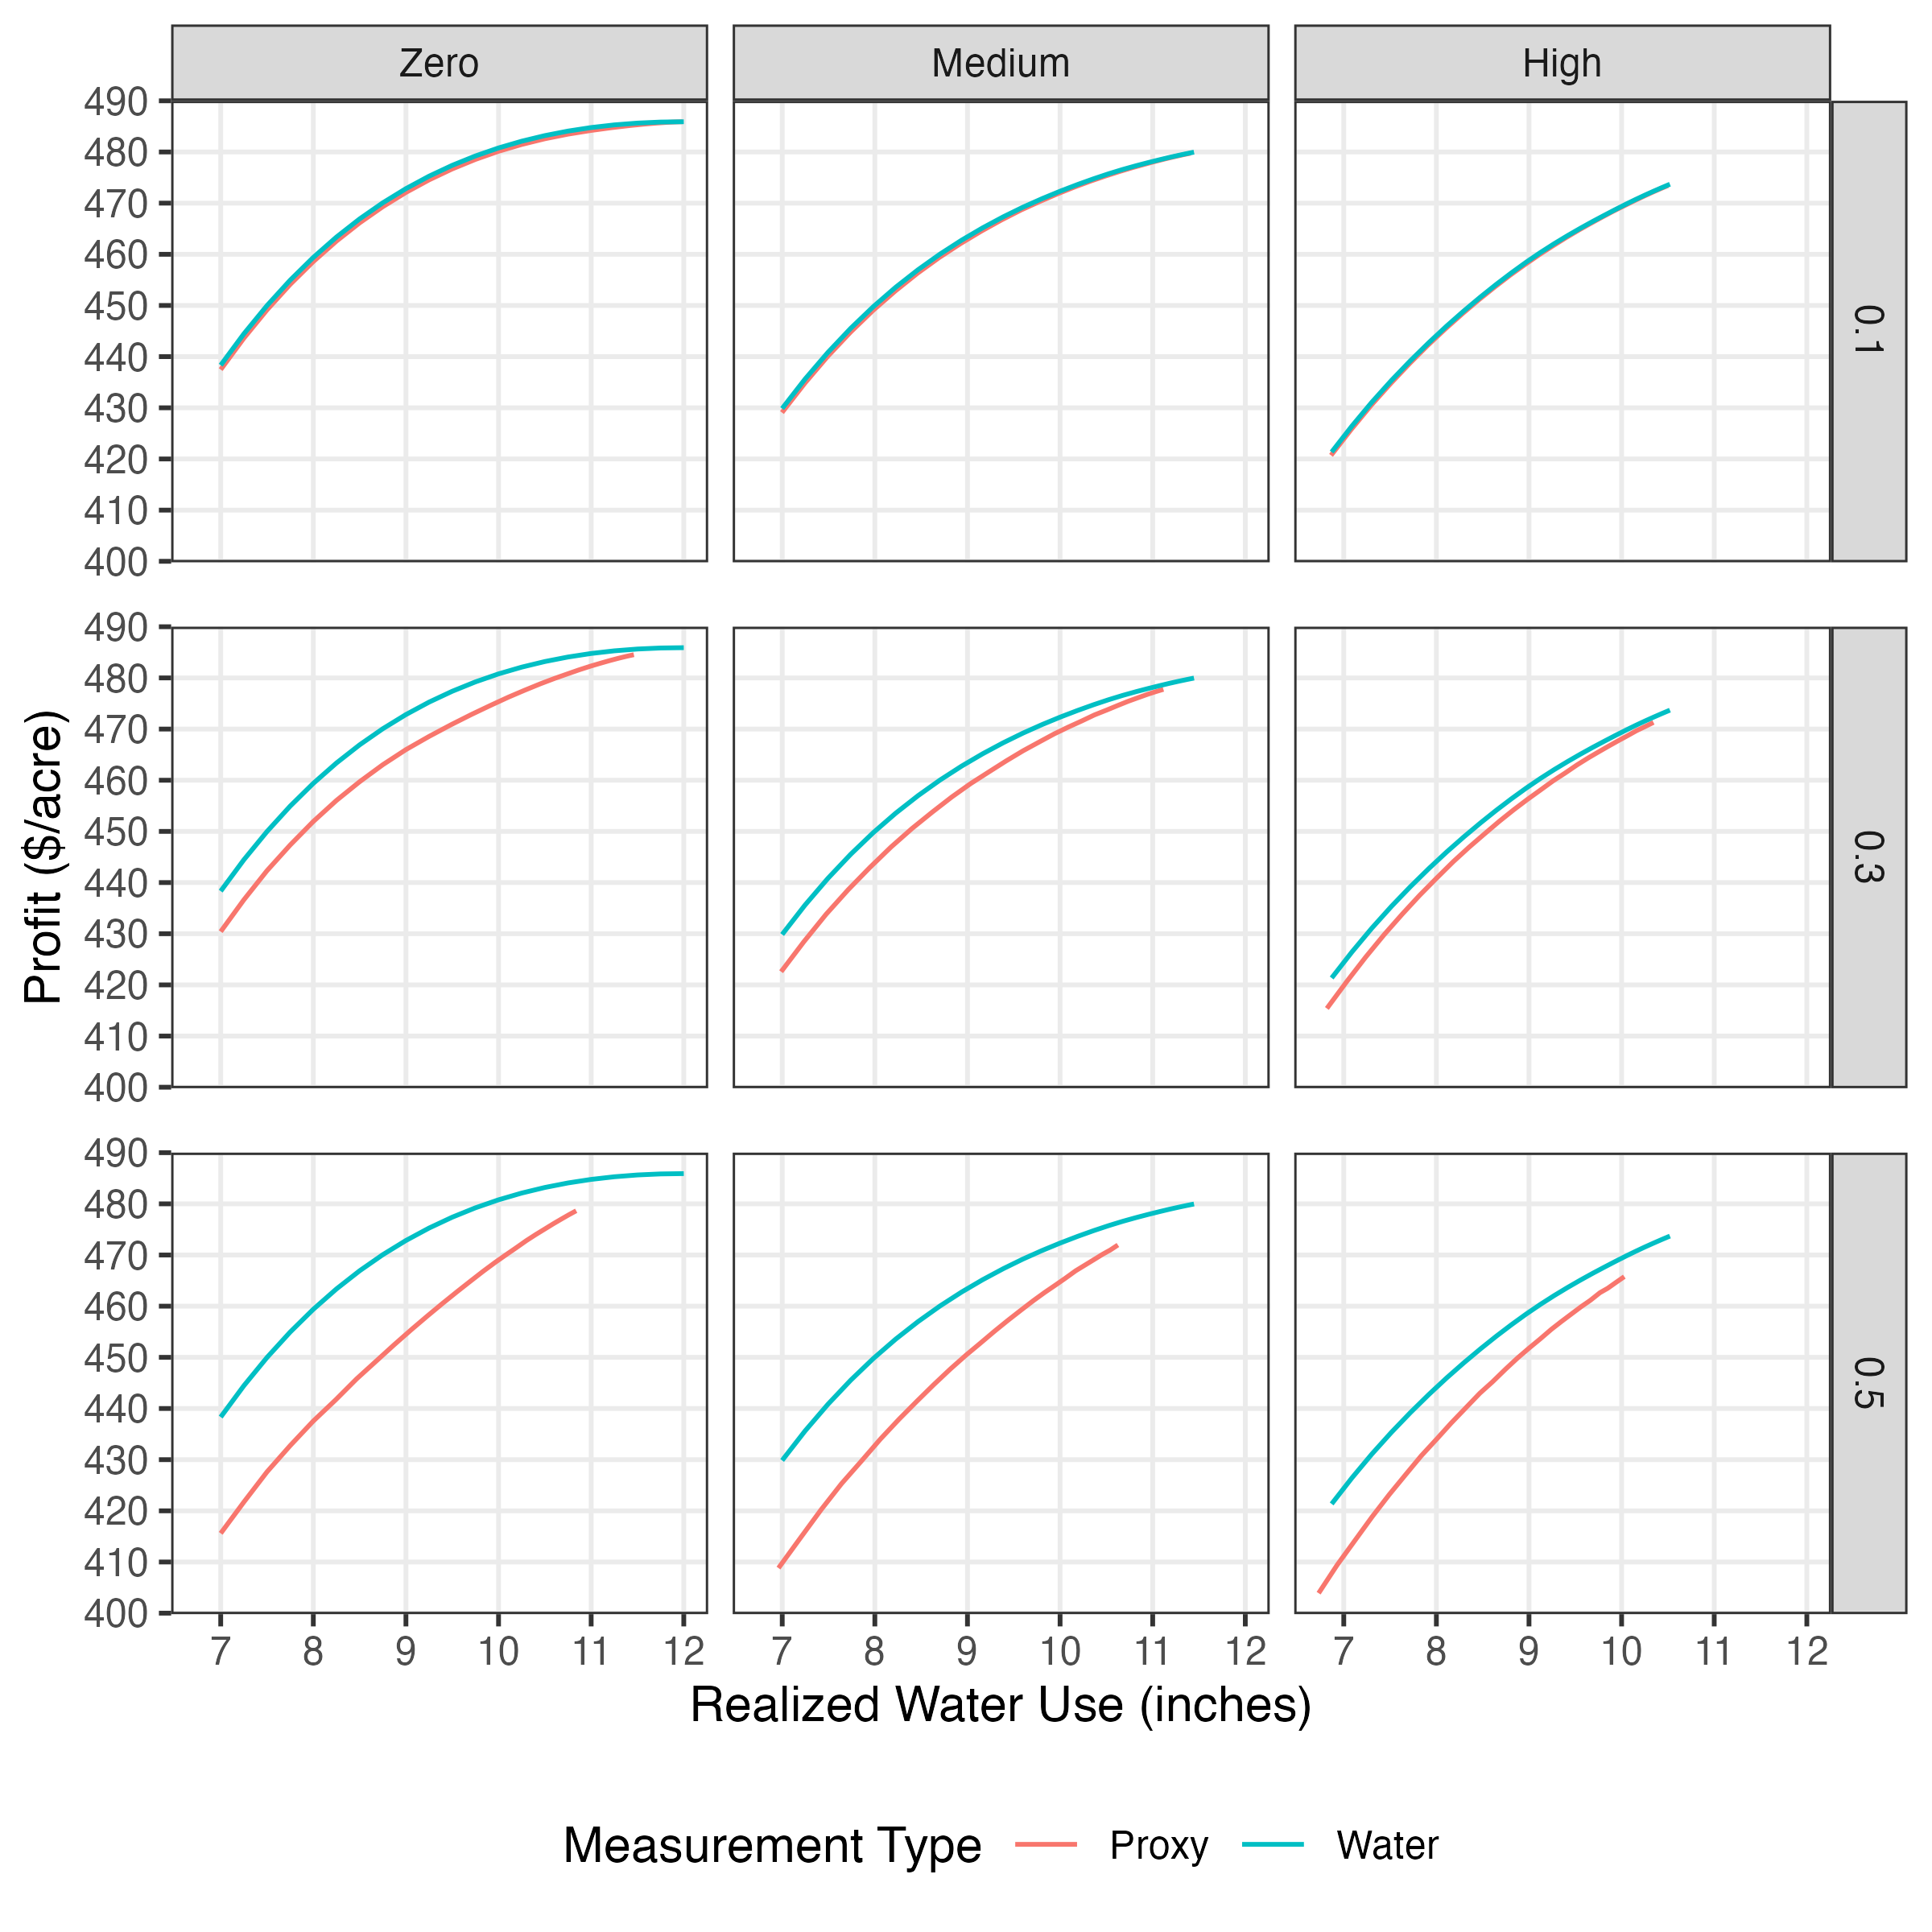
\includegraphics{figures/g_profit_quota_comp_stat} 

}

\caption{The impacts of an increase in the degree of measurement error on profit}\label{fig:increase-me-degree}
\end{figure}

\hypertarget{the-effect-of-allowing-trading-quota}{%
\subsection{The effect of allowing trading quota}\label{the-effect-of-allowing-trading-quota}}

Allowing quota to be traded among farmers can dramatically change the relative performance of the water- and quota-based regulation. Figure \ref{fig:trading-profit} presents profit for water-based quota, proxy-based quota, water-based quota trading, and proxy-based quota trading regulation systems. As shown in the figure, the disadvantage of using proxy almost disappears when trading of quota is allowed. This is because the inefficiencies in quota allocations are resolved through trading of quota whether it is water or proxy quota. (before trading and after trading?)

\begin{figure}[H]

{\centering 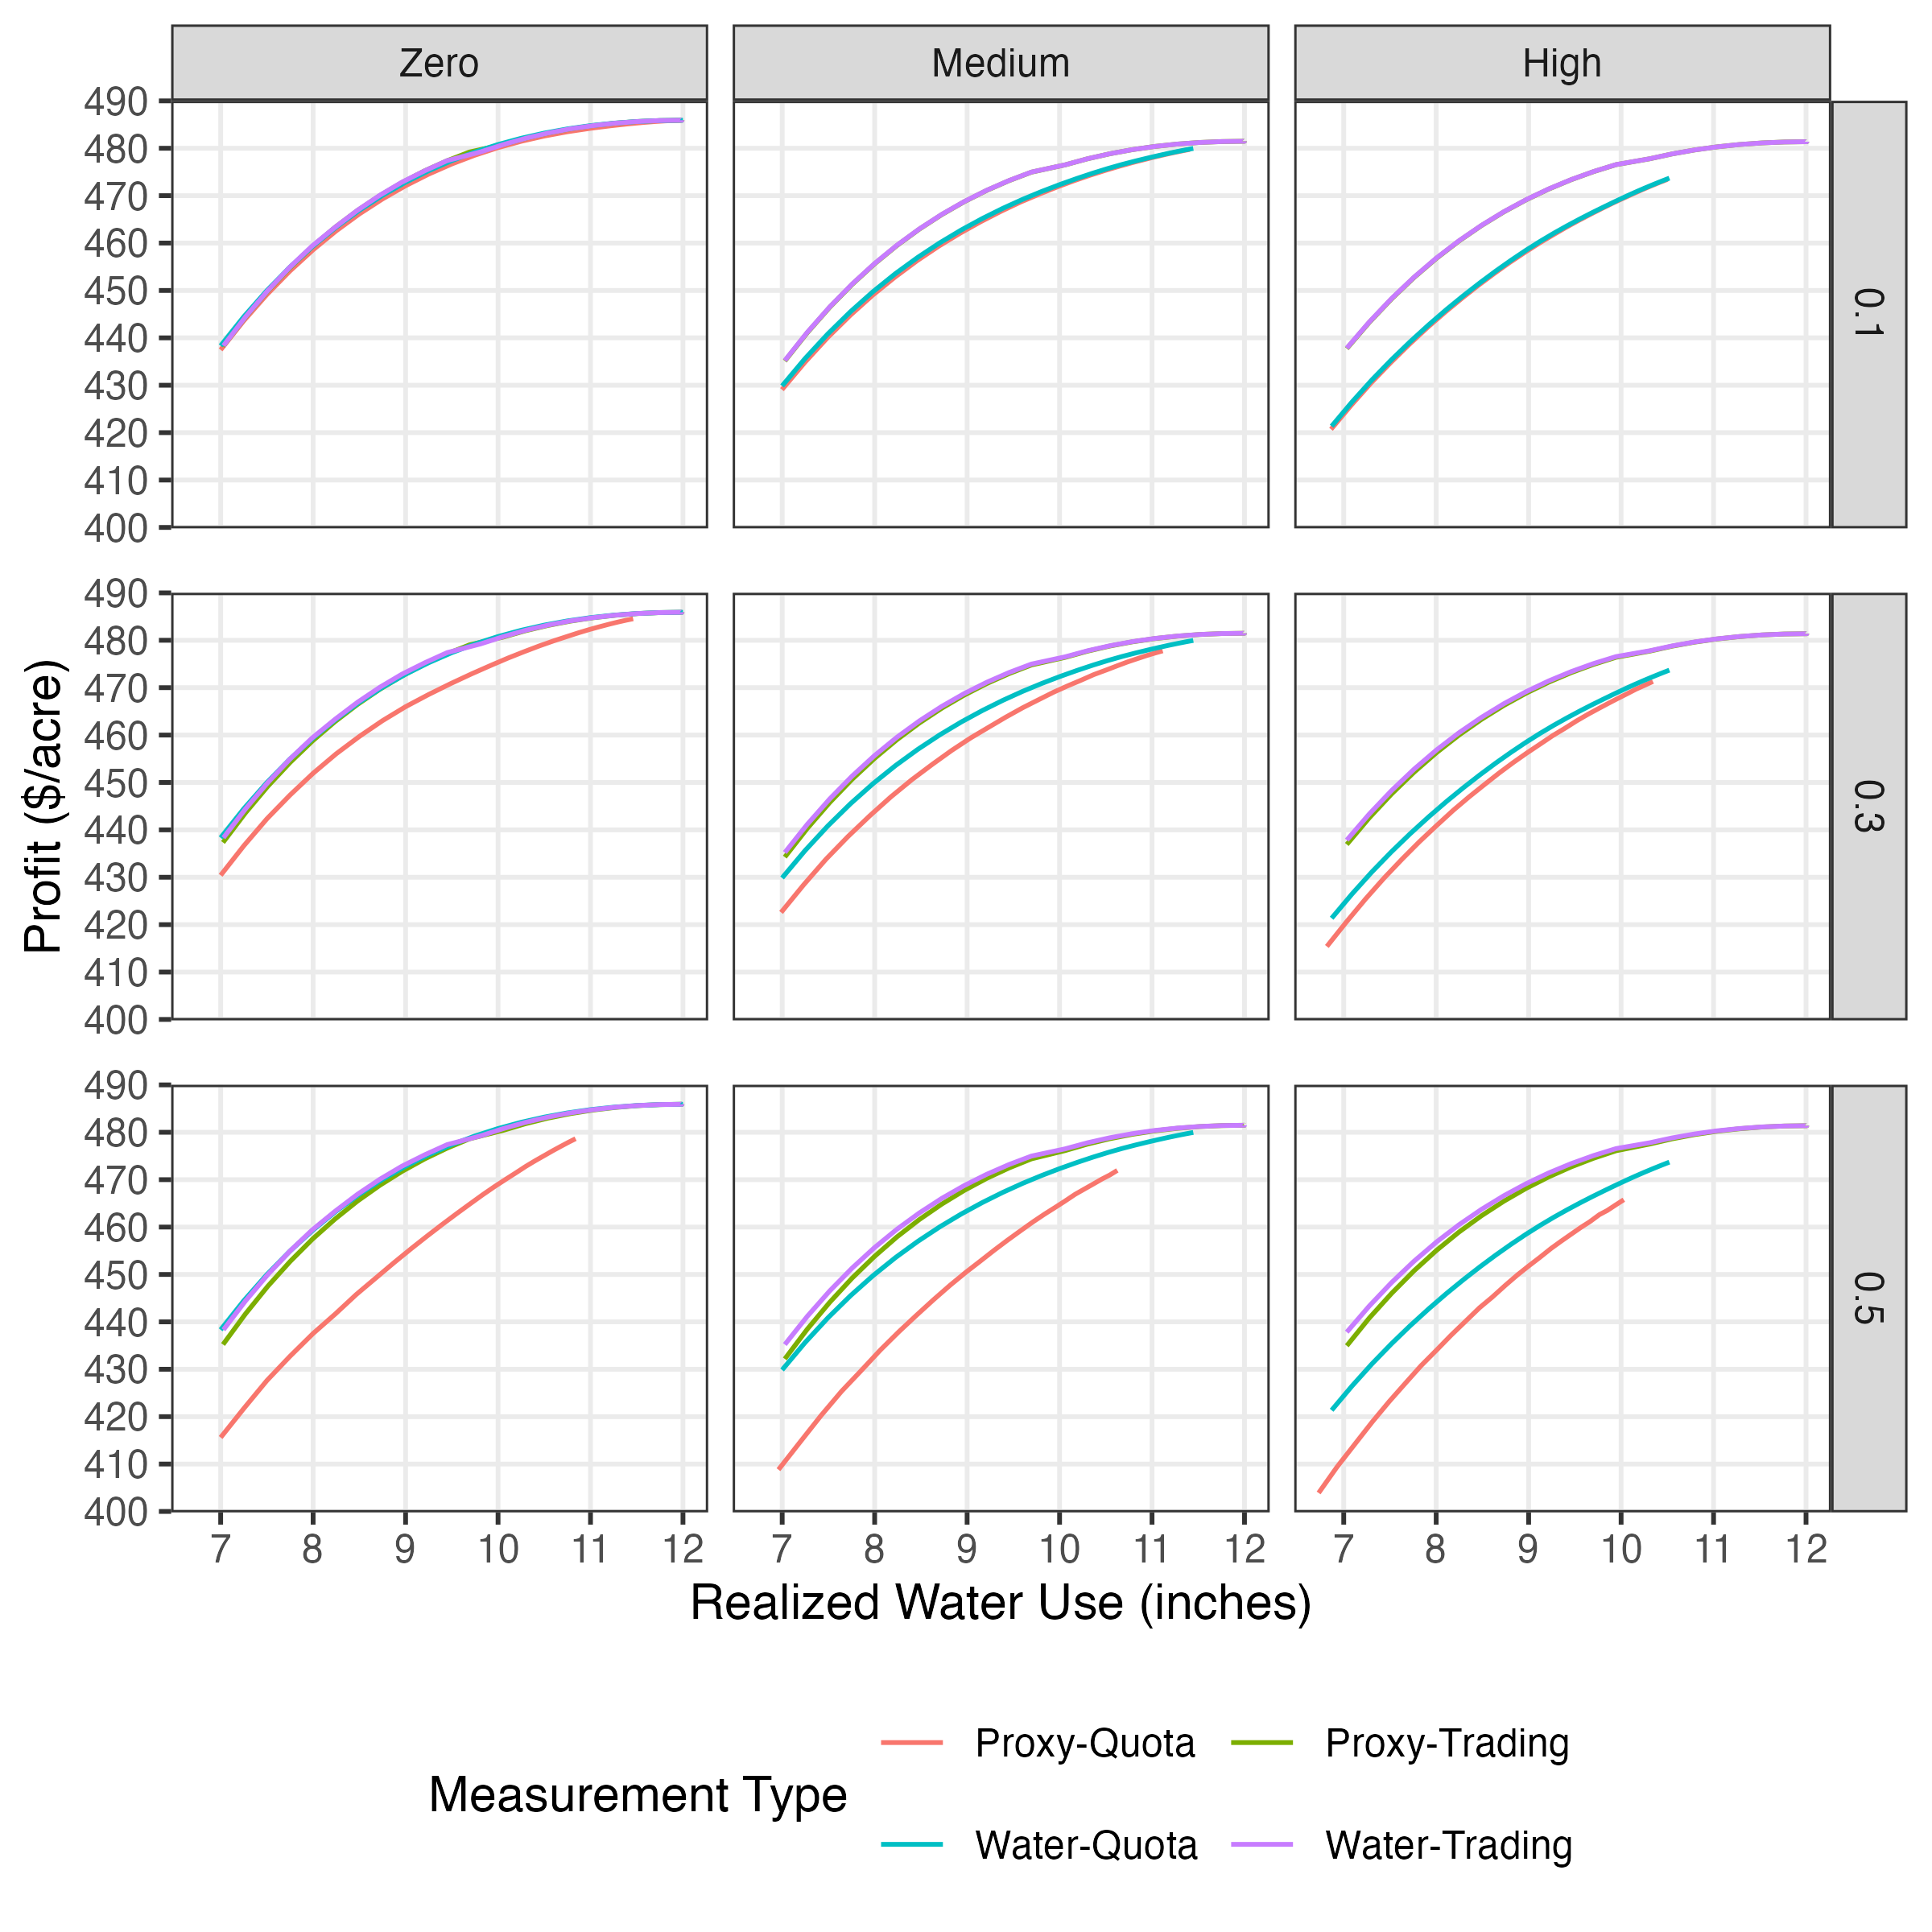
\includegraphics{figures/g_trade_effect_profit} 

}

\caption{Comparison of profit from agricultural production between the water and quota systems when quota trading is allowed}\label{fig:trading-profit}
\end{figure}

Figure \ref{fig:trading-profit-illustration} illustrates

While water-quota and proxy-quota trading perform about the same, water-quota always leads to a higher total profit for a given level of realized water use. In other words, to achieve a certain water use goal, water-quota trading is always to more cost-effective than proxy-quota trading. Under water-quota trading, the margial profit of water is equalized across the farmers, which is a necessary condition to achieve the highest profit for a given level of total water use. Under proxy-quota trading, the marginal profit of proxy is equalized across the farmers, not the margial profit of water (See Appendix \ldots{} for a mathematical proof). However, it is worth emphasizing that the inefficiency caused by the use of proxy is likely to be minimal as shown in Figure \ref{fig:trading-profit}.

\hypertarget{use-of-proxy-can-damage-distributional-equity}{%
\subsection{Use of proxy can damage distributional equity}\label{use-of-proxy-can-damage-distributional-equity}}

Figure \ref{fig:distributional-equity} presents the cumulative probability of the ratio of profit under quota-based relative to water-based system for quota (red) and permit trading (blue). Ratio of less than 1 indicates making less profit under the quota-based system compared to the water-based system. If farmers make just as much profir under proxy-based regulation compared to water-based regulation, then the cumulative probability line would be a vertical line at 1. For example, under the high degree of measurement error and medium heterogenenity scenario, some farmers would make about the half of what they would make under the water quota system. At the lower end of the distribution are farmers who would be constrained severely by water use quota, but whose water use estiamtes are much higher than their actual water use. At the higher end of the distribution are farmers who would be constrained by water use quota, but whose water use estiamtes are much lower than their actual water use. Famres who suffer significantly under the quota system can develop strong dissatisfaction of the quota-based regulation system, which in turn may lead to installing water meter themselves. If they discover the over-estimation of their water use, they may appeal to legal actions against the administrator for their unfair treatment. Allowind quota trading greatly diminishes the distributional inequality, though not completely. This is because unfortunate farmers who suffered from over-estimation of their water use can now at least purchase proxy quota to increase their production level.

\begin{figure}[H]

{\centering 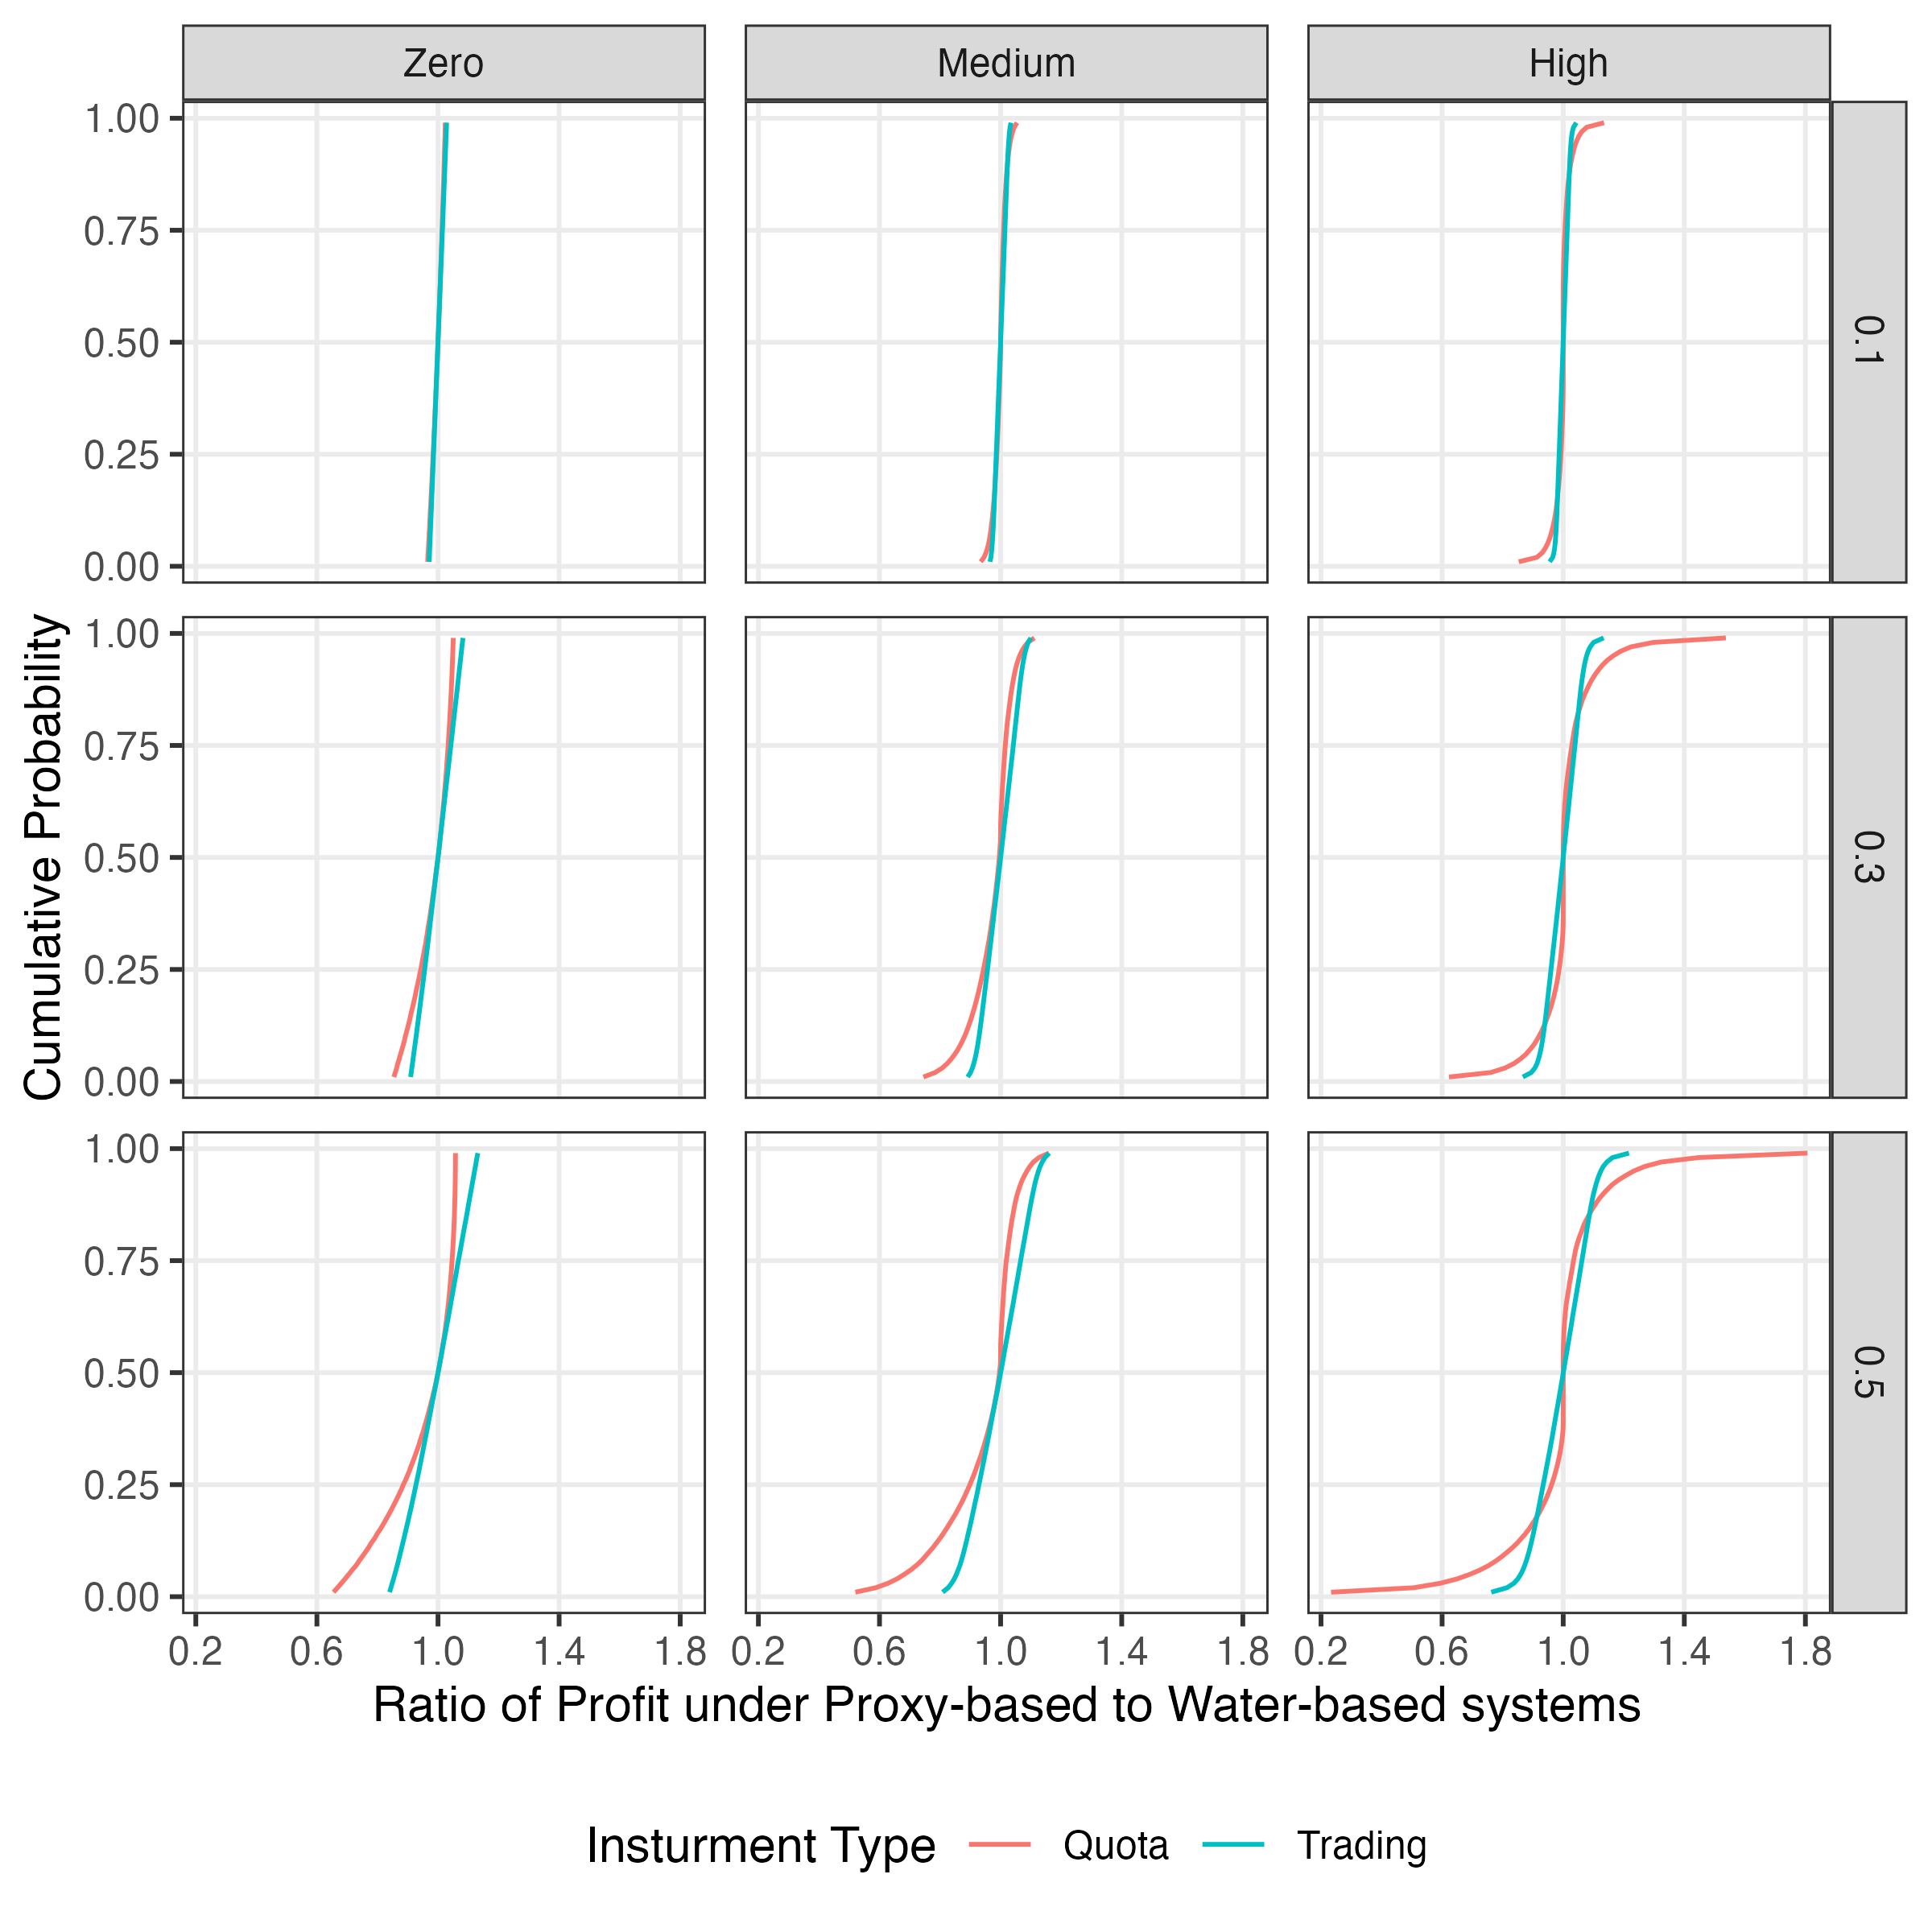
\includegraphics{figures/g_profit_ratio} 

}

\caption{Distribution of profit under various regulation systems}\label{fig:distributional-equity}
\end{figure}

\hypertarget{discussion}{%
\section{Discussion}\label{discussion}}

\hypertarget{limitations}{%
\subsection{Limitations}\label{limitations}}

Assumptions.
Temporal

\hypertarget{methods}{%
\section{Methods}\label{methods}}

\hypertarget{section}{%
\subsection{}\label{section}}

Assumptions:
+ farmers: has learned the degree of under- or over-estimation of water use compared to actual over the years and has learned how to irrigate up to the water use quota

\hypertarget{data-and-code-availability}{%
\subsection{Data and Code Availability}\label{data-and-code-availability}}

The datasets created in this article are all computer-generated using R codes. All the datasets and codes are available at .

\clearpage

\hypertarget{appendix-appendix}{%
\appendix}


\hypertarget{distribution-of-optimal-water-use-under-no-water-use-constraints}{%
\subsection{Distribution of optimal water use under no water use constraints}\label{distribution-of-optimal-water-use-under-no-water-use-constraints}}

\begin{figure}[H]

{\centering 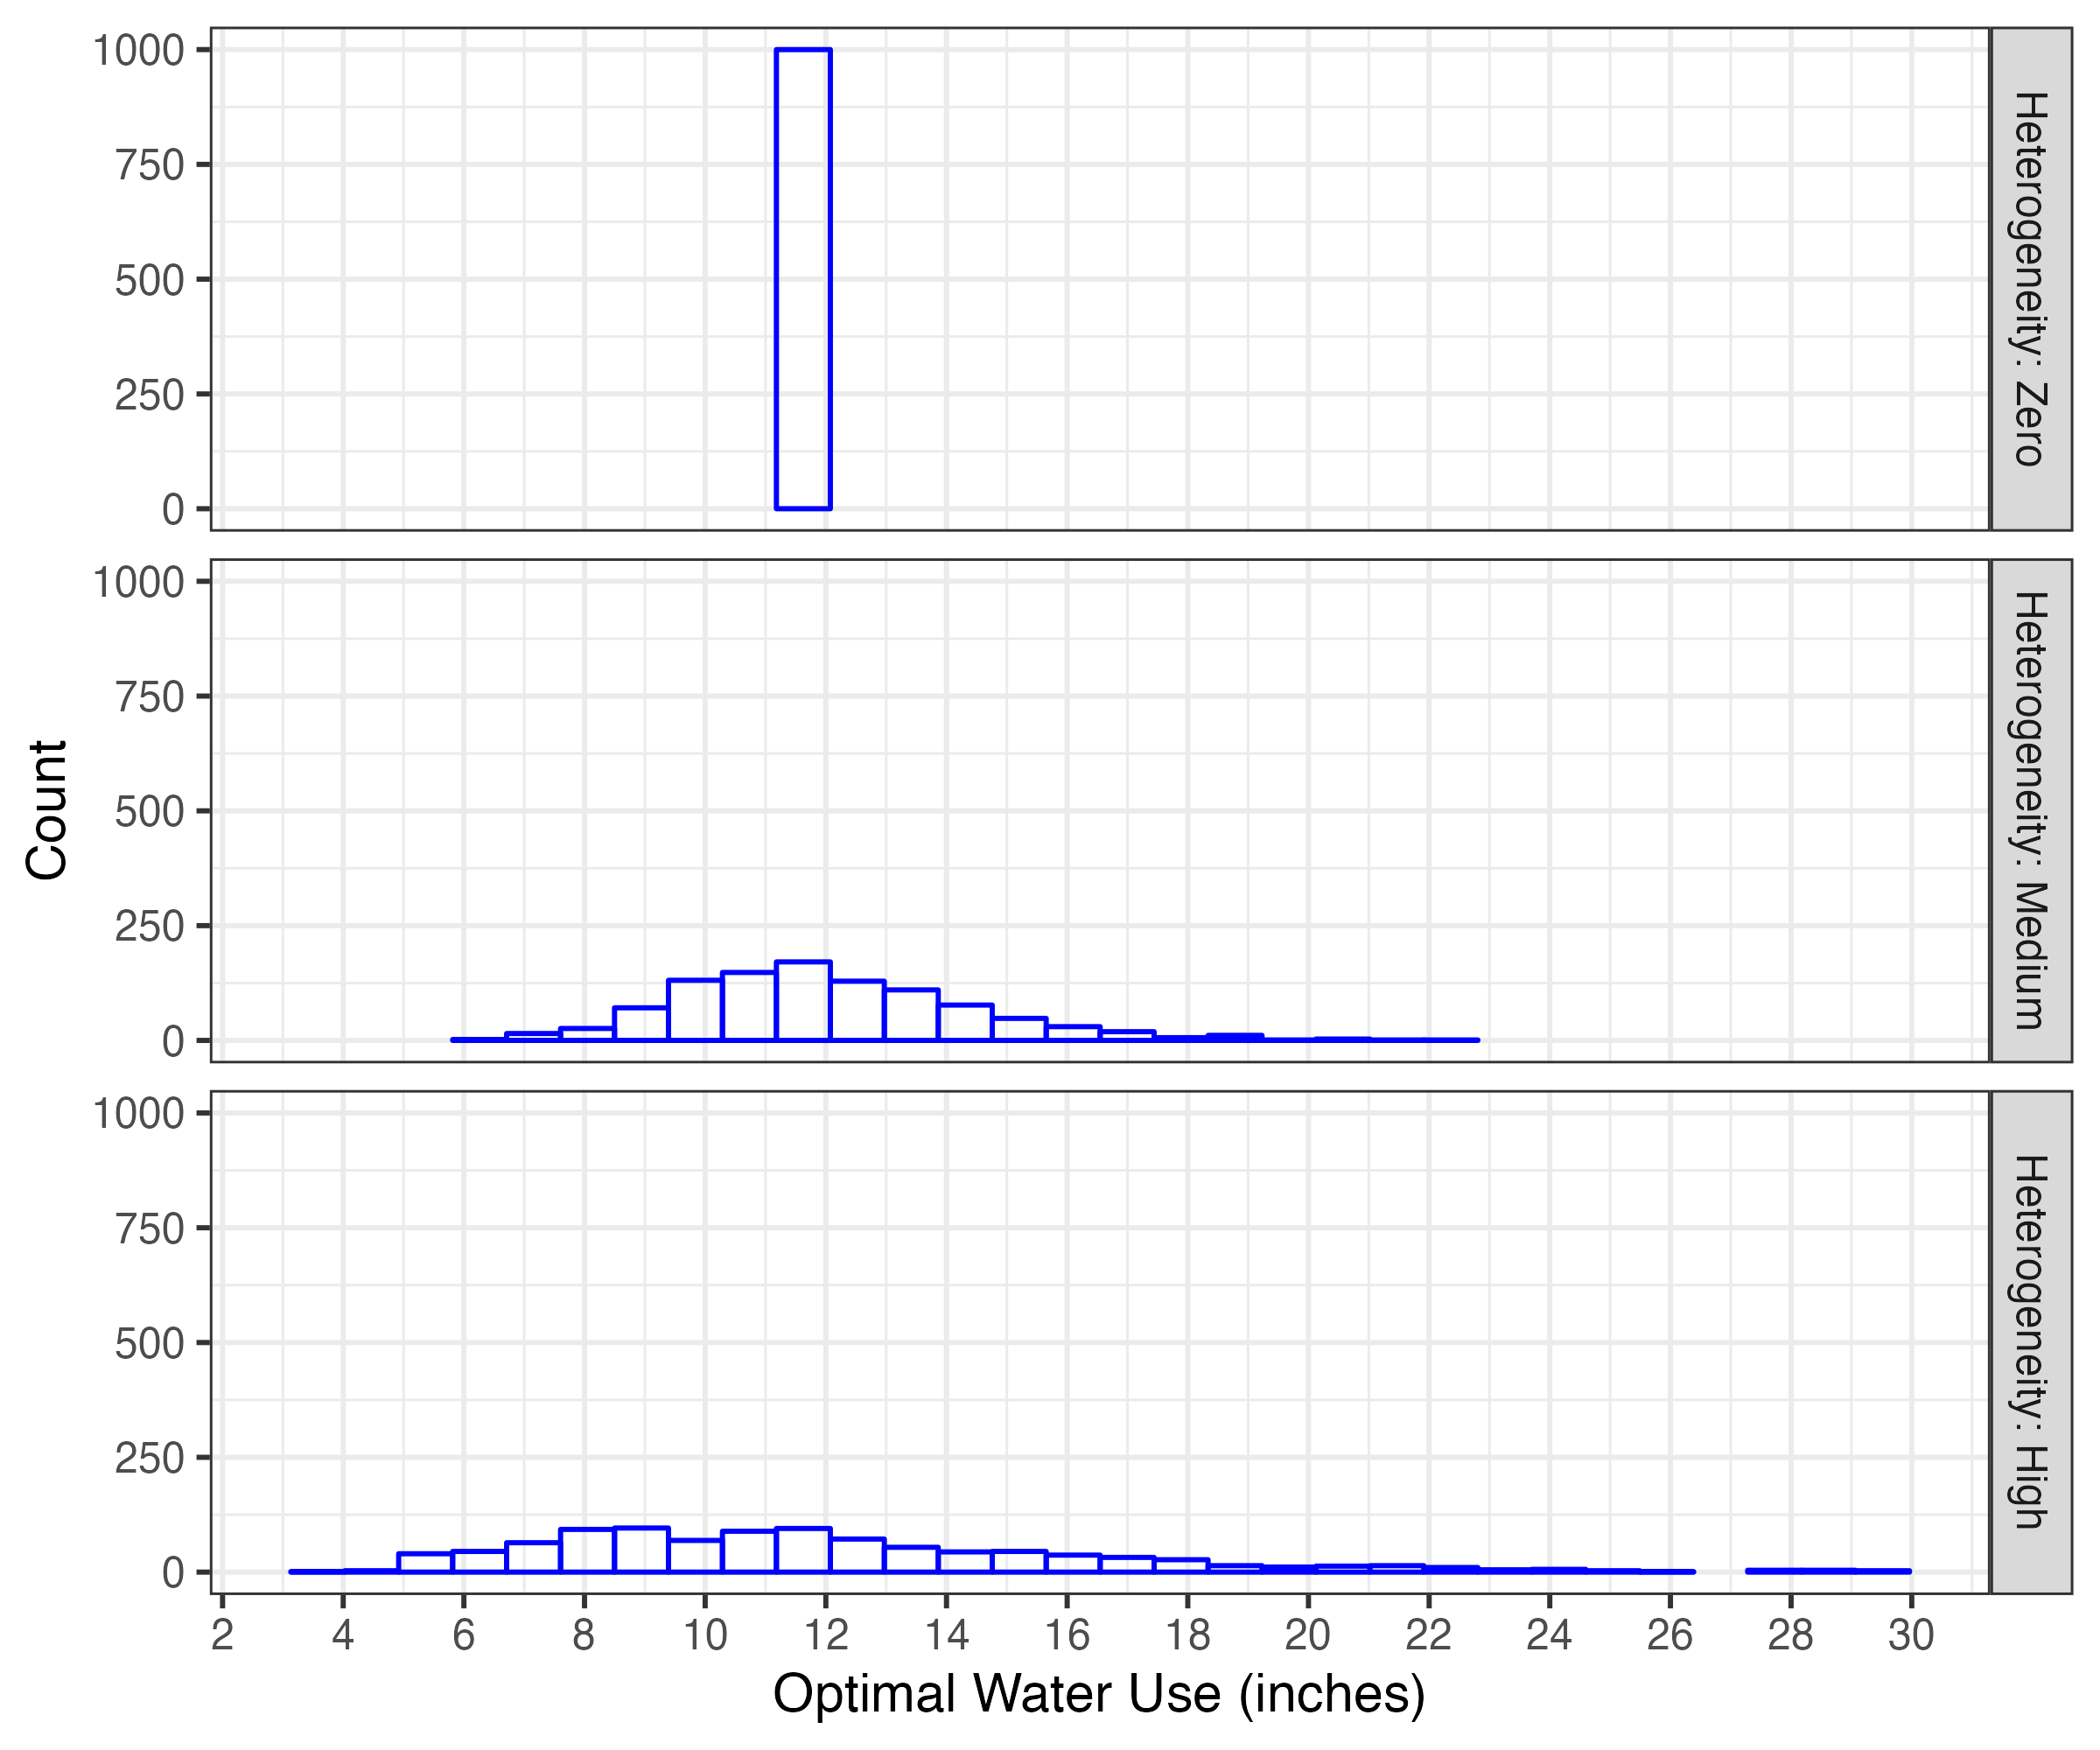
\includegraphics{figures/g_opt_w_dist} 

}

\caption{Distribution of optimal water use under no water use constraints}\label{fig:dist-opt-w}
\end{figure}

  \bibliography{DRA.bib}

\end{document}
